
\documentclass[letterpaper,12pt]{article}
 
\usepackage[spanish]{babel}
\usepackage[utf8]{inputenc}
\usepackage{listings}
\usepackage{graphicx}
 
%%%%%%%%%%%%%%%%%%%%%%%%%%% PORTADA %%%%%%%%%%%%%%%%%%%%%%%%%%%%%%%%%%%%%%%
\makeatletter
\def\thickhrulefill{\leavevmode \leaders \hrule height 1pt\hfill \kern \z@}
\renewcommand{\maketitle}{\begin{titlepage}%
    \let\footnotesize\small
    \let\footnoterule\relax
    \parindent \z@
    \reset@font
    \null\vfil
    \begin{flushleft}    
      \small \@curso \par
      \huge{\textbf{\@title}} \par
    \end{flushleft}
    \par
    \hrule height 4pt
    \par
    \begin{flushright}
      \Huge{\textbf{\@author}} \par
      \bigskip
      \normalsize{\@primerautor} \par
      \normalsize{\@segundoautor} \par
      \bigskip
      \bigskip
      \normalsize \@date \par
    \end{flushright}
    \vskip 60\p@
    \vfil\null
  \end{titlepage}%
  \setcounter{footnote}{0}%
}
\def\primerautor#1{\def\@primerautor{#1}}
\def\segundoautor#1{\def\@segundoautor{#1}}
\def\curso#1{\def\@curso{#1}}
\makeatother
%%%%%%%%%%%%%%%%%%%%%%%%%%% PORTADA %%%%%%%%%%%%%%%%%%%%%%%%%%%%%%%%%%%%%%%
 
 
 
%%%%%%%%%%%%%%%%%%%%%%%%%%% DATOS PERSONALES %%%%%%%%%%%%%%%%%%%%%%%
\curso{CC4102 Dise\~no y An\'alisis de Algoritmos}
\title{Informe Tarea II}
 
\primerautor{Agust\'in L\'opez Q.}
\segundoautor{Mat\'ias Cisterna M.}
 
 
 
\begin{document}
 
\maketitle
 
 
\newpage
\thispagestyle{empty}
\tableofcontents
\setcounter{page}{0}
\newpage
 
\section{Introducción}
En esta tarea 2 de Diseño y Análisis de Algoritmos se busca analizar el desempeño de búsqueda en diferentes estructuras de datos. Las estructuras a analizar son las siguientes: Árbol Binario de Búsqueda, Árbol AVL, Árbol de Van Emde Boas, Splay Tree y Árbol Optimo.
 
Un árbol binario de búsqueda (ABB) es una estructura de datos basada en nodos en forma de árbol. Es un árbol binario (solo puede haber hasta dos nodos hijos por padre), en el que todo a la izquierda del nodo padre es menor que el y todo a la derecha de el es mayor.

Un árbol AVL, es un árbol que cumple las características de un árbol binario de búsqueda. Sin embargo este tiene la particularidad de auto balancearse. Esto quiere decir que que la altura de las ramas del lado izquierdo no difieren en mas de una unidad de altura de la derecha.

Un árbol de Van Emde Boas (vEB tree), es una estructura de datos basada en arreglos asociativos en forma de árbol. En que todas sus operaciones son en el orden $(\log \left(\log M \right))$ siendo M el numero máximo de elementos que la estructura puede contener.

Un Splay tree es un árbol con las mismas características que un árbol AVL y con la singularidad de que los elementos accesados recientemente tienen mejor tiempo de acceso que el resto. Esto se logra mediante haciendo \textit{splaying} al elemento del árbol. Esto consiste en reordenar el árbol para que ese elemento quede mas arriba, logrando así menores tiempos de acceso. 

Un árbol de búsqueda optima es un árbol de búsqueda binaria. Con la excepción de que cuando se genera el árbol uno sabe de antemano cuales son las frecuencias de acceso de cada elemento. Con dicha información uno puede generar un árbol en que los elementos mas accesados estén antes, mejorando así los tiempos de acceso.

~\\
Características del Computador Usado:
\begin{itemize}
\item Cpu: Intel I7 x980 3.33Ghz
\item Ram: 8Gb ddr3 800Mhz
\item Disco duro: Sata II
\item Memoria JVM: 8Gb
\end{itemize}
\newpage 
\section{Hipótesis}
Se cree que tanto \textit{ABB}, \textit{AVL Trees} y \textit{Splay Trees} se comportaran de manera similar en su tiempo promedio de búsqueda. Sin embargo, en estas tres estructuras se espera diferentes tiempos de búsqueda en su peor caso. Por otro lado, para \textit{Van Emde Boas tree} Su tiempo de búsqueda va a depender estrictamente de el tamaño M con que se cree el árbol. Aun así este árbol, a menos que $M>>>N$ (siendo n el numero de elementos), debería tener mejores tiempos de acceso que el resto de los mencionados anteriormente. Finalmente se espera que el \textit{Optimal Binary Search Tree} posea el menor tiempo de acceso de búsqueda de todos los arboles.

\newpage
\section{Dise\~no Experimental}
\subsection{Implementaci\'on}
Para la implementaci\'on se us\'o el lenguaje de programaci\'on Java. El dise\~no se dividi\'o en 9 clases:

\begin{itemize}
\item \textit{ABBTree}: Representa al árbol binario de búsqueda.
\item \textit{AVLTree}: Representa al árbol AVL.
\item \textit{AVLNode}: Representa los nodos del árbol AVL.
\item \textit{IAVLNode}: Representa los nodos internos del árbol AVL.
\item \textit{NullAVLNode}: Representa los nodos nullos del árbol AVL.
\item \textit{SplayTree}: Representa al SplayTree.
\item \textit{vEBTree}: Representa al árbol de Van Emde Boas.
\item \textit{OpABBTree}:

\item \textit{StopWatch}: Clase creada para medir tiempos de forma simple.
\item \textit{Main}: Clase con m\'etodo \textit{main}, es desde donde se obtiene los datos.
\end{itemize}


Para la representación de cada estructura de datos: \textit{ABBTree}, \textit{AVLTree}, \textit{SplayTree}, \textit{vEBTree} y \textit{optimum ABBTree} se genero una clase que los representa. Dentro de cada clase se encuentra un método de inserción y búsqueda. Para las estructuras de datos Splay tree y AVL existen otros métodos que garantizan sus propiedades especificas de auto balanceo y nodos recién utilizados.

\begin{itemize}
\item B\'usqueda: Los algoritmos de búsqueda respectivamente para las 5 estructuras de datos reciben como parámetro un dato y retorna si se encuentra en la estructura o no y el tiempo que se demoro.

\item Inserción: Los algoritmos de inserción dependen exclusivamente de la estructura en que se este ejecutando. Aun así todos reciben un nuevo dato a insertar y estos retornan la nueva estructura de datos con la nueva inserción.

\begin{enumerate}
  \item \textit{ABBTree}: El método de inserción es bastante simple el árbol inserta el nuevo dato en su posición correspondiente fijándose en cumplir que todo lo que este a su izquierda sea menor a el y a su derecha mayor a el. Esto se cumple para todo nodo en el árbol.
  \item \textit{AVLTree}: El método de inserción cumple las mismas condiciones que el \textit{ABBTree} pero ademas este tiene que estar balanceado en su altura. Es decir la diferencia de altura de la rama mas larga con la rama mas corta es a lo mas una unidad.
  \item \textit{SplayTree}: El método de inserción cumple las mismas condiciones que el \textit{AVLTree} pero ademas este reorganiza el elemento que tuvo el ultimo accesados para que así si se busca ese mismo elemento sea mas rápido.
   \item \textit{vEBTree}: El método de inserción de esta estructura difiere al resto. Esto se debe a que el árbol esta concedido por arreglos y no por nodos. La inserción funciona de la siguiente manera: Si el arreglo esta vació los valores min y max son iguales al nuevo elemento. Si no, si $x<T.min$ entonces insertamos T.min al sub-árbol i responsable de T.min y T.min es ahora igual a x.Si no, si $x>T.max$ insertamos x en el sub-árbol i y T.max ahora es x. Finalmente si $T.min<x<T.max$ insertamos x en el sub-árbol i.
   \item \textit{OpABBTree}:
   
\end{enumerate}
\end{itemize}


\subsection{Generaci\'on de Instancias}

Se generan conjuntos de tamaños $ n \in$\{$2^{10},....2^{20}$\}. Ademas cada llave sera un numero natural que esta en el rango $ U = $\{$2^{10},....2^{20}$\}. Para cada $n$, se genera un conjunto al azar $K_n$ de $n$ llaves en el rango $U$. Finalmente se generan secuencias de tamaño $100n$ sobre estas llaves de tres maneras distintas al azar:
\begin{itemize}

\item \textbf{Distribución 1}: Se escogen $100n$ números al azar entre el conjunto de llaves $K_n$.

\item \textbf{Distribución 2}: Se escoge que la $i$-esima llave aparece con probabilidad $c/i^a$, donde $c$ es una constante de normalización. $ a \in$\{1.2,1.5,2.0\}.

\item \textbf{Distribución 3}: Se escoge que la $i$-esima llave aparece con probabilidad $c/a^i$, donde $c$ es una constante de normalización. $ a \in$\{1.2,1.5,2.0\}.

Finalmente el bloque de código de la creación de las 3 distribuciones queda así:

\lstset{language=Java, breaklines=true, basicstyle=\footnotesize}
\begin{lstlisting}[frame=single, numbersep=5pt, numbers=left, tabsize=3] 
for(int n=1024;n <= 1024*1024; n*=2)
{
	potencia = (int)(Math.log(n)/Math.log(2));
	Kn = new int[n];
	seq1 = new int[100*n];
	seq2 = new int[3][100*n];
	seq3 = new int[3][100*n];
	freq1 = new double[100*n];
	freq2 = new double[3][100*n];
	freq3 = new double[3][100*n];
	for (int i = 0; i < n; i++) 
	{
		Kn[i] = r.nextInt(U) + 1;
	}
	// secuencia 1
	for (int i = 0; i < 100*n; i++) 
	{
		seq1[i] = Kn[r.nextInt(n)];
		freq1[i] = 1.0/(100*n);
	}
	// secuencia 2 
	int i = 0;
	int k = 0;
	for(int index=0;index<3;index++)
	{
		double c = getC2(a[index],n);
		while(i <= 100*n)
		{				
			double freq_k = c/Math.pow(k+1,a[index]); // frecuencia de Kn[k]
			int cant_k = (int)Math.ceil(100*n*freq_k); // cantidad de Kn[k]
			for(int j=i;j<(100*n) && j<(i+cant_k);j++)
			{
				seq2[index][j] = Kn[k];
				freq2[index][j] = freq_k;
			}
			k++;
			i += cant_k;
		}			
	// 	secuencia 3 
		i = 0;
		k = 0;
		c = getC3(a[index],n);
		while(i <= 100*n)
		{
			double freq_k = c/Math.pow(a[index],k+1); // frecuencia de Kn[k]
			int cant_k = (int)Math.ceil(100*n*freq_k); // cantidad de Kn[k]
			for(int j=i;j<(100*n) && j<(i+cant_k);j++)
			{
				seq3[index][j] = Kn[k];
				freq3[index][j] = freq_k;
			}
			k++;
			i += cant_k;
		}
	}
}	
\end{lstlisting}

\end{itemize}



\subsection{Medidas de Rendimiento}
Las medidas de rendimiento usadas son dos en base al tiempo:
\begin{itemize}

\item Primero es el tiempo de demora en la construcción de cada estructura en cuestión.
	
\item Segundo es el tiempo de demora en la búsqueda de un elemento en cada estructura.

\end{itemize}

Finalmente estas medidas, tanto de búsqueda como de inserción, son almacenadas en un nuevo archivo. Creado con el objetivo de almacenar los datos y luego analizarlos.

\newpage
\section{Presentación de Resultados}

\subsection{Datos}
A continuación se presentan los resultados obtenidos según la distribución de creación de datos usada.

\subsubsection{Distribución 1}

\begin{tabular}{|c|c|c|c|c|}
\hline
\textbf{$n$} & \textbf{Tipo Árbol} & \textbf{T/P Construcción (ms)} & \textbf{T/P Búsqueda (ms)} \\
\hline
10 & ABBTree & 0.0 & 0.0 \\
\hline
10 & AVLTree & 9.765625E-5 & 9.765625E-5 \\
\hline
10 & vEBTree & 5.859375E-4 & 1.953125E-4 \\
\hline
10 & SplayTree & 0.0 & 1.953125E-4 \\
\hline
\hline
11 & ABBTree & 3.90625E-4 & 1.46484375E-4 \\
\hline
11 & AVLTree & 1.46484375E-4 & 1.46484375E-4 \\
\hline
11 & vEBTree & 2.44140625E-4 & 9.765625E-5\\
\hline
11 & SplayTree & 2.44140625E-4 & 3.41796875E-4 \\
\hline
\hline
12 & ABBTree & 9.765625E-5  & 1.220703125E-4  \\
\hline
12 & AVLTree & 2.2216796875E-4 & 4.8828125E-5 \\
\hline
12 & vEBTree & 2.197265625E-4 & 9.765625E-5\\
\hline
12 & SplayTree & 2.4658203125E-4 & 9.765625E-5 \\
\hline
\hline
13 & ABBTree & 1.46484375E-4 & 1.8310546875E-4  \\
\hline
13 & AVLTree & 2.5634765625E-4 & 1.220703125E-5 \\
\hline
13 & vEBTree & 1.5869140625E-4 & 1.0986328125E-4 \\
\hline
13 & SplayTree & 3.173828125E-4 & 1.708984375E-4 \\
\hline
\hline
14 & ABBTree & 2.79541015625E-4 & 1.568603515625E-4 \\
\hline
14 & AVLTree & 2.74658203125E-4 & 3.35693359375E-5 \\
\hline
14 & vEBTree & 2.72216796875E-4 & 9.3994140625E-5\\
\hline
14 & SplayTree & 2.685546875E-4 & 2.130126953125E-4 \\
\hline
\hline
15 & ABBTree & 2.8533935546875E-4 & 1.7333984375E-4 \\
\hline
15 & AVLTree & 3.2012939453125E-4 & 2.8076171875E-5 \\
\hline
15 & vEBTree & 2.911376953125E-4  & 1.2939453125E-4\\
\hline
15 & SplayTree & 4.16259765625E-4 & 2.7069091796875E-4 \\
\hline
\end{tabular}

\begin{tabular}{|c|c|c|c|c|}
\hline
\textbf{$n$} & \textbf{Tipo Árbol} & \textbf{T/P Construcción (ms)} & \textbf{T/P Búsqueda (ms)} \\
\hline
16 & ABBTree & 3.26385498046875E-4 & 1.98822021484375E-4 \\
\hline
16 & AVLTree & 3.95965576171875E-4  & 3.96728515625E-5 \\
\hline
16 & vEBTree & 2.99835205078125E-4  & 1.66015625E-4 \\
\hline
16 & SplayTree & 4.91943359375E-4  & 3.05328369140625E-4 \\
\hline
\hline
17 & ABBTree & 4.718780517578125E-4  & 4.317474365234375E-4 \\
\hline
17 & AVLTree & 4.55322265625E-4  & 4.67681884765625E-5 \\
\hline
17 & vEBTree & 4.058074951171875E-4  & 1.99737548828125E-4\\
\hline
17 & SplayTree & 6.873321533203125E-4 & 6.812286376953125E-4 \\
\hline
\hline
18 & ABBTree & 6.123733520507813E-4 & 5.675506591796875E-4 \\
\hline
18 & AVLTree & 5.17425537109375E-4 & 5.3253173828125E-5 \\
\hline
18 & vEBTree & 4.06646728515625E-4 & 2.39715576171875E-4 \\
\hline
18 & SplayTree & 9.239578247070313E-4  & 8.881378173828125E-4 \\
\hline
\hline
19 & ABBTree & 4.918670654296875E-4 & 4.2222976684570313E-4 \\
\hline
19 & AVLTree & 6.448554992675781E-4  & 4.358291625976563E-5 \\
\hline
19 & vEBTree & 3.5610198974609373E-4 & 2.5114059448242185E-4\\
\hline
19 & SplayTree & 8.919906616210938E-4 & 7.759475708007812E-4 \\
\hline
\hline
20 & ABBTree & 5.703926086425781E-4 & 4.689788818359375E-4 \\
\hline
20 & AVLTree & 7.653236389160156E-4 & 3.966331481933594E-5 \\
\hline
20 & vEBTree & 4.260730743408203E-4 & 3.116989135742187E-4\\
\hline
20 & SplayTree & 9.851646423339844E-4 & 7.950210571289062E-4 \\
\hline
\end{tabular}
\\ \\

\subsubsection{Distribución 2 ($a=1.2$)}

\begin{tabular}{|c|c|c|c|c|}
\hline
\textbf{$n$} & \textbf{Tipo Árbol} & \textbf{T/P Construcción (ms)} & \textbf{T/P Búsqueda (ms)} \\
\hline
10 & ABBTree & 9.765625E-5 & 0.0 \\
\hline
10 & AVLTree & 9.765625E-5 & 9.765625E-5 \\
\hline
10 & vEBTree & 9.765625E-5 & 0.0\\
\hline
10 & SplayTree & 0.0 & 0.0 \\
\hline
\hline
11 & ABBTree & 9.765625E-5 & 9.765625E-5 \\
\hline
11 & AVLTree & 9.765625E-5 & 1.953125E-4 \\
\hline
11 & vEBTree & 4.8828125E-5 & 1.46484375E-4\\
\hline
11 & SplayTree & 9.765625E-5 & 0.0 \\
\hline
\hline
12 & ABBTree & 2.44140625E-5 & 0.0  \\
\hline
12 & AVLTree & 4.8828125E-5 & 9.765625E-5 \\
\hline
12 & vEBTree & 4.8828125E-5 & 0.0\\
\hline
12 & SplayTree & 2.44140625E-5 & 0.0 \\
\hline
\hline
13 & ABBTree & 2.44140625E-5 & 3.662109375E-5  \\
\hline
13 & AVLTree & 4.8828125E-5 & 1.220703125E-5 \\
\hline
13 & vEBTree & 4.8828125E-5 & 2.44140625E-5\\
\hline
13 & SplayTree & 2.44140625E-5 & 2.44140625E-5 \\
\hline
\hline
14 & ABBTree & 2.9296875E-5 & 1.8310546875E-5 \\
\hline
14 & AVLTree & 5.92041015625E-5 & 2.3193359375E-5 \\
\hline
14 & vEBTree & 5.18798828125E-5 & 2.62451171875E-5\\
\hline
14 & SplayTree & 1.77001953125E-5 & 3.35693359375E-5 \\
\hline
\hline
15 & ABBTree & 3.204345703125E-5 & 2.899169921875E-5 \\
\hline
15 & AVLTree & 5.43212890625E-5 & 2.105712890625E-5 \\
\hline
15 & vEBTree & 6.16455078125E-5  & 2.960205078125E-5\\
\hline
15 & SplayTree & 2.13623046875E-5 & 1.922607421875E-5 \\
\hline
\end{tabular}

\begin{tabular}{|c|c|c|c|c|}
\hline
\textbf{$n$} & \textbf{Tipo Árbol} & \textbf{T/P Construcción (ms)} & \textbf{T/P Búsqueda (ms)} \\
\hline
16 & ABBTree & 3.4332275390625E-5 & 4.180908203125E-5 \\
\hline
16 & AVLTree & 5.7830810546875E-5  & 2.288818359375E-5 \\
\hline
16 & vEBTree & 5.8746337890625E-5  & 3.0517578125E-5 \\
\hline
16 & SplayTree & 1.6937255859375E-5 & 1.983642578125E-5 \\
\hline
\hline
17 & ABBTree & 3.62396240234375E-5  & 2.49481201171875E-5 \\
\hline
17 & AVLTree & 6.15692138671875E-5 & 3.7994384765625E-5 \\
\hline
17 & vEBTree & 5.51605224609375E-5  & 3.7841796875E-5\\
\hline
17 & SplayTree & 2.23541259765625E-5 & 2.5177001953125E-5 \\
\hline
\hline
18 & ABBTree & 3.490447998046875E-5 & 3.078460693359375E-5 \\
\hline
18 & AVLTree & 5.863189697265625E-5 & 4.413604736328125E-5 \\
\hline
18 & vEBTree & 5.970001220703125E-5 & 3.41033935546875E-5 \\
\hline
18 & SplayTree & 2.197265625E-5  & 2.7008056640625E-5 \\
\hline
\hline
19 & ABBTree & 3.795623779296875E-5 & 3.017425537109375E-5 \\
\hline
19 & AVLTree & 6.336212158203125E-5  & 2.3021697998046876E-5 \\
\hline
19 & vEBTree & 7.328033447265625E-5 & 4.0798187255859376E-5\\
\hline
19 & SplayTree & 2.758026123046875E-5 & 2.407073974609375E-5 \\
\hline
\hline
20 & ABBTree & 3.759384155273438E-5 & 3.063201904296875E-5 \\
\hline
20 & AVLTree & 6.516456604003906E-5 & 3.787994384765625E-5 \\
\hline
20 & vEBTree & 5.89752197265625E-5 & 3.6401748657226564E-5\\
\hline
20 & SplayTree & 2.541542053222656E-5 & 2.3603439331054688E-5 \\
\hline
\end{tabular}
\\ \\

\subsubsection{Distribución 2 ($a=1.5$)}

\begin{tabular}{|c|c|c|c|c|}
\hline
\textbf{$n$} & \textbf{Tipo Árbol} & \textbf{T/P Construcción (ms)} & \textbf{T/P Búsqueda (ms)} \\
\hline
10 & ABBTree & 0.0 & 0.0 \\
\hline
10 & AVLTree & 9.765625E-5 & 0.0 \\
\hline
10 & vEBTree & 9.765625E-5 & 1.953125E-4\\
\hline
10 & SplayTree & 0.0 & 9.765625E-5 \\
\hline
\hline
11 & ABBTree & 0.0 & 4.8828125E-5  \\
\hline
11 & AVLTree & 0.0 & 0.0 \\
\hline
11 & vEBTree & 1.46484375E-4 & 8.45721739062895E-5\\
\hline
11 & SplayTree & 0.0 & 0.0 \\
\hline
\hline
12 & ABBTree & 0.0 4 & 2.44140625E-5  \\
\hline
12 & AVLTree & 2.685546875E-4 & 0.0 \\
\hline
12 & vEBTree & 1.5869140625E-4 & 4.8828125E-5\\
\hline
12 & SplayTree & 0.0 & 0.0 \\
\hline
\hline
13 & ABBTree & 1.220703125E-5 & 1.220703125E-5  \\
\hline
13 & AVLTree & 1.220703125E-5 & 3.662109375E-5 \\
\hline
13 & vEBTree & 6.103515625E-5 & 1.220703125E-5\\
\hline
13 & SplayTree & 2.44140625E-5 & 2.44140625E-5 \\
\hline
\hline
14 & ABBTree & 3.41796875E-5 & 2.13623046875E-5 \\
\hline
14 & AVLTree & 1.3427734375E-55 & 1.03759765625E-5 \\
\hline
14 & vEBTree & 4.5166015625E-5 & 1.77001953125E-5\\
\hline
14 & SplayTree & 1.15966796875E-5 & 1.46484375E-5 \\
\hline
\hline
15 & ABBTree & 2.105712890625E-5 & 1.434326171875E-5 \\
\hline
15 & AVLTree & 1.617431640625E-5 & 1.251220703125E-5 \\
\hline
15 & vEBTree & 4.913330078125E-5  & 2.197265625E-5\\
\hline
15 & SplayTree & 2.685546875E-5 & 1.708984375E-5 \\
\hline
\end{tabular}

\begin{tabular}{|c|c|c|c|c|}
\hline
\textbf{$n$} & \textbf{Tipo Árbol} & \textbf{T/P Construcción (ms)} & \textbf{T/P Búsqueda (ms)} \\
\hline
16 & ABBTree & 1.5869140625E-5 & 1.5869140625E-5 \\
\hline
16 & AVLTree & 1.739501953125E-5  & 9.613037109375E-6 \\
\hline
16 & vEBTree & 5.0506591796875E-5  & 1.3427734375E-5 \\
\hline
16 & SplayTree & 1.617431640625E-5 & 2.62451171875E-5 \\
\hline
\hline
17 & ABBTree & 1.73187255859375E-5  & 1.678466796875E-5 \\
\hline
17 & AVLTree & 1.8463134765625E-5 & 1.54876708984375E-5 \\
\hline
17 & vEBTree & 4.60052490234375E-5  & 1.617431640625E-5\\
\hline
17 & SplayTree & 1.6937255859375E-5 & 2.01416015625E-5 \\
\hline
\hline
18 & ABBTree & 1.8463134765625E-5 & 1.544952392578125E-5 \\
\hline
18 & AVLTree & 1.743316650390625E-5 & 1.708984375E-5  \\
\hline
18 & vEBTree & 5.08880615234375E-5 & 1.79290771484375E-5 \\
\hline
18 & SplayTree & 1.922607421875E-5  & 2.063751220703125E-5 \\
\hline
\hline
19 & ABBTree & 1.6956329345703126E-5 & 1.781463623046875E-5 \\
\hline
19 & AVLTree & 1.827239990234375E-5  & 1.556396484375E-5 \\
\hline
19 & vEBTree & 5.208969116210937E-5 & 1.3713836669921876E-5\\
\hline
19 & SplayTree & 1.8215179443359376E-5  & 1.598358154296875E-5 \\
\hline
\hline
20 & ABBTree & 1.7251968383789062E-5 & 1.729011535644531E-5 \\
\hline
20 & AVLTree & 1.6269683837890624E-5 & 1.5249252319335938E-5 \\
\hline
20 & vEBTree & 5.316734313964844E-5  & 1.8024444580078124E-5\\
\hline
20 & SplayTree & 1.560211181640625E-54 & 1.739501953125E-5 \\
\hline
\end{tabular}
\\ \\

\subsubsection{Distribución 2 ($a=2.0$)}

\begin{tabular}{|c|c|c|c|c|}
\hline
\textbf{$n$} & \textbf{Tipo Árbol} & \textbf{T/P Construcción (ms)} & \textbf{T/P Búsqueda (ms)} \\
\hline
10 & ABBTree & 0.0 & 0.0 \\
\hline
10 & AVLTree & 0.0 & 0.0 \\
\hline
10 & vEBTree & 9.765625E-5 & 9.765625E-5\\
\hline
10 & SplayTree & 0.0 & 0.0 \\
\hline
\hline
11 & ABBTree & 0.0 & 0.0  \\
\hline
11 & AVLTree & 0.0 & 0.0 \\
\hline
11 & vEBTree & 9.765625E-5 & 6.90530594244522E-5\\
\hline
11 & SplayTree & 0.0 & 9.765625E-5 \\
\hline
\hline
12 & ABBTree & 4.8828125E-5 & 2.44140625E-5  \\
\hline
12 & AVLTree & 0.0 & 4.8828125E-5 \\
\hline
12 & vEBTree & 7.32421875E-5 & 2.44140625E-5\\
\hline
12 & SplayTree & 0.0 & 4.8828125E-5 \\
\hline
\hline
13 & ABBTree & 1.220703125E-5 & 0.0  \\
\hline
13 & AVLTree & 2.44140625E-5 & 0.0 \\
\hline
13 & vEBTree & 3.662109375E-5 & 3.662109375E-5 \\
\hline
13 & SplayTree & 1.220703125E-5 & 2.44140625E-5  \\
\hline
\hline
14 & ABBTree & 2.197265625E-5 & 1.5869140625E-5 \\
\hline
14 & AVLTree & 1.40380859375E-5 & 1.5869140625E-5 \\
\hline
14 & vEBTree & 4.45556640625E-5 & 2.685546875E-5\\
\hline
14 & SplayTree & 3.173828125E-5 & 2.197265625E-5 \\
\hline
\hline
15 & ABBTree & 1.46484375E-5 & 2.13623046875E-5 \\
\hline
15 & AVLTree & 2.3193359375E-5 & 1.46484375E-5 \\
\hline
15 & vEBTree & 4.7607421875E-5  & 1.312255859375E-5\\
\hline
15 & SplayTree & 1.434326171875E-5 & 1.617431640625E-5 \\
\hline
\end{tabular}

\begin{tabular}{|c|c|c|c|c|}
\hline
\textbf{$n$} & \textbf{Tipo Árbol} & \textbf{T/P Construcción (ms)} & \textbf{T/P Búsqueda (ms)} \\
\hline
16 & ABBTree & 1.6937255859375E-5 & 1.9378662109375E-5 \\
\hline
16 & AVLTree & 2.25830078125E-5 & 1.0833740234375E-5 \\
\hline
16 & vEBTree & 5.1116943359375E-5 & 1.3427734375E-5 \\
\hline
16 & SplayTree & 2.105712890625E-5 & 1.9378662109375E-5 \\
\hline
\hline
17 & ABBTree & 2.32696533203125E-5  & 1.88446044921875E-5 \\
\hline
17 & AVLTree & 2.46429443359375E-5 & 1.3275146484375E-5 \\
\hline
17 & vEBTree & 4.81414794921875E-5  & 1.6326904296875E-5\\
\hline
17 & SplayTree & 1.30462646484375E-5 & 2.0294189453125E-5 \\
\hline
\hline
18 & ABBTree & 1.773834228515625E-5 & 1.85394287109375E-5 \\
\hline
18 & AVLTree & 1.796722412109375E-5 & 1.216888427734375E-5 \\
\hline
18 & vEBTree & 4.852294921875E-5 & 1.79290771484375E-5 \\
\hline
18 & SplayTree & 1.857757568359375E-5  & 1.834869384765625E-5 \\
\hline
\hline
19 & ABBTree & 1.89971923828125E-5 & 1.6632080078125E-5 \\
\hline
19 & AVLTree & 1.65557861328125E-5  & 1.407623291015625E-5 \\
\hline
19 & vEBTree & 4.871368408203125E-5 & 1.5850067138671876E-5\\
\hline
19 & SplayTree & 1.8596649169921875E-5 & 2.01416015625E-5 \\
\hline
\hline
20 & ABBTree & 1.633644104003906E-5 & 1.5869140625E-5 \\
\hline
20 & AVLTree & 1.9235610961914064E-5 & 1.4352798461914063E-5 \\
\hline
20 & vEBTree & 4.763603210449219E-5 & 1.4886856079101562E-5\\
\hline
20 & SplayTree & 1.6880035400390624E-5 & 1.6374588012695314E-5 \\
\hline
\end{tabular}
\\ \\

\subsubsection{Distribución 3 ($a=1.2$)}

\begin{tabular}{|c|c|c|c|c|}
\hline
\textbf{$n$} & \textbf{Tipo Árbol} & \textbf{T/P Construcción (ms)} & \textbf{T/P Búsqueda (ms)} \\
\hline
10 & ABBTree & 9.765625E-5 & 1.953125E-4 \\
\hline
10 & AVLTree & 1.953125E-4 & 0.0 \\
\hline
10 & vEBTree & 9.765625E-5 & 9.765625E-5\\
\hline
10 & SplayTree & 0.0  & 0.0 \\
\hline
\hline
11 & ABBTree & 4.8828125E-5 & 0.0 \\
\hline
11 & AVLTree & 4.8828125E-5 & 9.765625E-5 \\
\hline
11 & vEBTree &  4.8828125E-5 & 4.8828125E-5\\
\hline
11 & SplayTree & 4.8828125E-5 & 0.0 \\
\hline
\hline
12 & ABBTree & 0.0 & 2.44140625E-5  \\
\hline
12 & AVLTree & 4.8828125E-5 & 2.44140625E-5 \\
\hline
12 & vEBTree & 2.44140625E-5 & 2.44140625E-55\\
\hline
12 & SplayTree & 0.0 & 0.0 \\
\hline
\hline
13 & ABBTree & 3.662109375E-5 & 1.220703125E-5   \\
\hline
13 & AVLTree & 3.662109375E-5 & 0.0 \\
\hline
13 & vEBTree & 8.544921875E-5 & 1.220703125E-5\\
\hline
13 & SplayTree & 3.662109375E-5 & 4.8828125E-5 \\
\hline
\hline
14 & ABBTree & 2.3193359375E-5 & 2.86865234375E-5 \\
\hline
14 & AVLTree & 3.23486328125E-5 & 2.62451171875E-5 \\
\hline
14 & vEBTree & 4.69970703125E-5 & 1.89208984375E-5\\
\hline
14 & SplayTree & 1.8310546875E-5 & 3.0517578125E-5 \\
\hline
\hline
15 & ABBTree & 1.8310546875E-5 & 1.52587890625E-5 \\
\hline
15 & AVLTree & 3.47900390625E-5 & 2.410888671875E-5 \\
\hline
15 & vEBTree & 4.669189453125E-5  & 2.62451171875E-5\\
\hline
15 & SplayTree & 2.166748046875E-5 & 2.9296875E-5 \\
\hline
\end{tabular}

\begin{tabular}{|c|c|c|c|c|}
\hline
\textbf{$n$} & \textbf{Tipo Árbol} & \textbf{T/P Construcción (ms)} & \textbf{T/P Búsqueda (ms)} \\
\hline
16 & ABBTree & 2.1209716796875E-5 & 1.617431640625E-5 \\
\hline
16 & AVLTree & 2.25830078125E-5  & 2.0904541015625E-5 \\
\hline
16 & vEBTree & 5.7830810546875E-5  & 1.8157958984375E-5 \\
\hline
16 & SplayTree & 2.13623046875E-5 & 1.7547607421875E-5 \\
\hline
\hline
17 & ABBTree & 2.0751953125E-5  & 2.41851806640625E-5 \\
\hline
17 & AVLTree & 2.47955322265625E-5 & 2.44140625E-5 \\
\hline
17 & vEBTree & 5.33294677734375E-5  & 2.0904541015625E-5\\
\hline
17 & SplayTree & 2.11334228515625E-5 & 2.09808349609375E-5 \\
\hline
\hline
18 & ABBTree & 2.7008056640625E-5 & 1.8463134765625E-5 \\
\hline
18 & AVLTree & 2.796173095703125E-5 & 2.552032470703125E-5 \\
\hline
18 & vEBTree & 5.207061767578125E-5 & 2.655029296875E-5 \\
\hline
18 & SplayTree & 2.208709716796875E-5  & 2.044677734375E-5 \\
\hline
\hline
19 & ABBTree & 2.368927001953125E-5 & 2.12860107421875E-5 \\
\hline
19 & AVLTree & 3.4332275390625E-5  & 2.6702880859375E-5 \\
\hline
19 & vEBTree & 5.67626953125E-5 & 2.1228790283203126E-5\\
\hline
19 & SplayTree & 1.80816650390625E-5 & 2.0503997802734375E-5 \\
\hline
\hline
20 & ABBTree & 2.3088455200195313E-5 & 2.020835876464844E-5 \\
\hline
20 & AVLTree & 2.6750564575195313E-5 & 2.26593017578125E-5 \\
\hline
20 & vEBTree & 5.1059722900390624E-5 & 2.482414245605469E-5\\
\hline
20 & SplayTree & 2.3860931396484375E-5 & 1.972198486328125E-5 \\
\hline
\end{tabular}
\\ \\

\subsubsection{Distribución 3 ($a=1.5$)}

\begin{tabular}{|c|c|c|c|c|}
\hline
\textbf{$n$} & \textbf{Tipo Árbol} & \textbf{T/P Construcción (ms)} & \textbf{T/P Búsqueda (ms)} \\
\hline
10 & ABBTree & 9.765625E-5 & 0.0 \\
\hline
10 & AVLTree & 1.953125E-4 & 9.765625E-5 \\
\hline
10 & vEBTree & 1.953125E-4 & 9.765625E-5\\
\hline
10 & SplayTree & 0.0 & 0.0 \\
\hline
\hline
11 & ABBTree & 0.0 & 4.8828125E-5 \\
\hline
11 & AVLTree & 9.765625E-5 & 0.0 \\
\hline
11 & vEBTree & 9.765625E-5 & 4.8828125E-5\\
\hline
11 & SplayTree & 0.0 & 4.8828125E-5 \\
\hline
\hline
12 & ABBTree & 0.0 & 0.0  \\
\hline
12 & AVLTree & 2.44140625E-5 & 2.44140625E-5 \\
\hline
12 & vEBTree & 1.46484375E-4 & 0.0\\
\hline
12 & SplayTree & 0.0 & 2.44140625E-5 \\
\hline
\hline
13 & ABBTree & 1.220703125E-5 & 3.662109375E-5  \\
\hline
13 & AVLTree & 2.44140625E-5 & 0.0 \\
\hline
13 & vEBTree & 4.8828125E-5 & 0.0\\
\hline
13 & SplayTree & 1.220703125E-5 & 4.8828125E-5 \\
\hline
\hline
14 & ABBTree & 2.3193359375E-5 & 1.8310546875E-5 \\
\hline
14 & AVLTree & 1.5869140625E-5 & 2.62451171875E-5 \\
\hline
14 & vEBTree & 4.5166015625E-5 & 2.50244140625E-5\\
\hline
14 & SplayTree & 2.197265625E-5 & 2.5634765625E-5 \\
\hline
\hline
15 & ABBTree & 1.89208984375E-5 & 1.708984375E-5 \\
\hline
15 & AVLTree & 2.227783203125E-5 & 2.3193359375E-5 \\
\hline
15 & vEBTree & 5.828857421875E-5  & 2.044677734375E-5\\
\hline
15 & SplayTree & 2.25830078125E-5 & 1.77001953125E-5 \\
\hline
\end{tabular}

\begin{tabular}{|c|c|c|c|c|}
\hline
\textbf{$n$} & \textbf{Tipo Árbol} & \textbf{T/P Construcción (ms)} & \textbf{T/P Búsqueda (ms)} \\
\hline
16 & ABBTree & 2.1209716796875E-5 & 1.7547607421875E-5 \\
\hline
16 & AVLTree & 3.387451171875E-5  & 3.11279296875E-5 \\
\hline
16 & vEBTree & 5.6610107421875E-5  & 1.2664794921875E-5 \\
\hline
16 & SplayTree & 2.044677734375E-5 & 1.861572265625E-5 \\
\hline
\hline
17 & ABBTree & 1.953125E-5  & 2.6397705078125E-5 \\
\hline
17 & AVLTree & 2.5177001953125E-5 & 1.71661376953125E-5 \\
\hline
17 & vEBTree & 4.95147705078125E-5  & 1.65557861328125E-5\\
\hline
17 & SplayTree & 1.922607421875E-5 & 2.3193359375E-5 \\
\hline
\hline
18 & ABBTree & 2.26593017578125E-5 & 2.0599365234375E-5 \\
\hline
18 & AVLTree & 2.086639404296875E-5 & 2.00653076171875E-5 \\
\hline
18 & vEBTree & 5.28717041015625E-5 & 2.03704833984375E-5 \\
\hline
18 & SplayTree & 2.048492431640625E-5  & 2.2125244140625E-5 \\
\hline
\hline
19 & ABBTree & 2.101898193359375E-5 & 2.2106170654296875E-5 \\
\hline
19 & AVLTree & 2.4967193603515625E-5  & 2.1610260009765625E-5 \\
\hline
19 & vEBTree & 5.37109375E-5 & 2.1266937255859376E-5\\
\hline
19 & SplayTree & 2.544403076171875E-5 & 2.14385986328125E-5 \\
\hline
\hline
20 & ABBTree & 2.1638870239257814E-5 & 2.0971298217773436E-5 \\
\hline
20 & AVLTree & 2.3908615112304688E-5 & 2.5539398193359376E-5 \\
\hline
20 & vEBTree & 5.372047424316406E-5 & 1.9121170043945313E-5\\
\hline
20 & SplayTree & 2.066612243652344E-5 & 2.0437240600585937E-5 \\
\hline
\end{tabular}
\\ \\

\subsubsection{Distribución 3 ($a=2.0$)}

\begin{tabular}{|c|c|c|c|c|}
\hline
\textbf{$n$} & \textbf{Tipo Árbol} & \textbf{T/P Construcción (ms)} & \textbf{T/P Búsqueda (ms)} \\
\hline
10 & ABBTree & 0.0 & 0.0 \\
\hline
10 & AVLTree & 0.0 & 9.765625E-5 \\
\hline
10 & vEBTree & 1.953125E-4 & 0.0\\
\hline
10 & SplayTree & 0.0 & 0.0 \\
\hline
\hline
11 & ABBTree & 9.765625E-5 & 8.30078125E-5 \\
\hline
11 & AVLTree & 0.0 & 0.0 \\
\hline
11 & vEBTree & 4.8828125E-5 & 4.8828125E-5 \\
\hline
11 & SplayTree & 0.0 & 0.0 \\
\hline
\hline
12 & ABBTree & 4.8828125E-5 & 2.44140625E-5  \\
\hline
12 & AVLTree & 2.44140625E-5 & 0.0 \\
\hline
12 & vEBTree & 4.8828125E-5 & 2.44140625E-5\\
\hline
12 & SplayTree & 0.0 & 0.0 \\
\hline
\hline
13 & ABBTree & 1.220703125E-5 & 4.8828125E-5  \\
\hline
13 & AVLTree & 2.44140625E-5 & 1.220703125E-5 \\
\hline
13 & vEBTree & 7.32421875E-5 & 1.220703125E-5\\
\hline
13 & SplayTree & 1.220703125E-5 & 0.0 \\
\hline
\hline
14 & ABBTree & 2.62451171875E-5 & 1.220703125E-5 \\
\hline
14 & AVLTree & 1.3427734375E-5 & 3.60107421875E-5 \\
\hline
14 & vEBTree & 7.14111328125E-5 & 1.46484375E-5\\
\hline
14 & SplayTree & 1.15966796875E-5 & 1.220703125E-5 \\
\hline
\hline
15 & ABBTree & 1.922607421875E-5 & 2.410888671875E-5 \\
\hline
15 & AVLTree & 2.01416015625E-5 & 2.197265625E-5 \\
\hline
15 & vEBTree & 6.65283203125E-5  & 1.373291015625E-5\\
\hline
15 & SplayTree & 1.953125E-5  & 1.678466796875E-5 \\
\hline
\end{tabular}

\begin{tabular}{|c|c|c|c|c|}
\hline
\textbf{$n$} & \textbf{Tipo Árbol} & \textbf{T/P Construcción (ms)} & \textbf{T/P Búsqueda (ms)} \\
\hline
16 & ABBTree & 1.800537109375E-5 & 1.434326171875E-5 \\
\hline
16 & AVLTree & 2.471923828125E-5  & 2.471923828125E-5 \\
\hline
16 & vEBTree & 5.8746337890625E-5  & 1.800537109375E-5 \\
\hline
16 & SplayTree & 1.7547607421875E-5 & 2.349853515625E-5 \\
\hline
\hline
17 & ABBTree & 1.861572265625E-5  & 1.97601318359375E-5 \\
\hline
17 & AVLTree & 1.6326904296875E-5 & 1.4801025390625E-5 \\
\hline
17 & vEBTree & 4.9591064453125E-5  & 1.8463134765625E-5\\
\hline
17 & SplayTree & 2.26593017578125E-5 & 2.12860107421875E-5 \\
\hline
\hline
18 & ABBTree & 2.4261474609375E-5 & 1.57928466796875E-5 \\
\hline
18 & AVLTree & 2.307891845703125E-5 & 2.124786376953125E-5 \\
\hline
18 & vEBTree & 5.59234619140625E-5 & 2.033233642578125E-5 \\
\hline
18 & SplayTree & 1.758575439453125E-5  & 2.09808349609375E-5 \\
\hline
\hline
19 & ABBTree & 1.842498779296875E-5 & 1.7642974853515625E-5 \\
\hline
19 & AVLTree & 2.513885498046875E-5  & 2.2258758544921875E-5 \\
\hline
19 & vEBTree & 5.3253173828125E-5 & 1.9741058349609374E-5\\
\hline
19 & SplayTree & 2.094268798828125E-5 & 1.949310302734375E-5 \\
\hline
\hline
20 & ABBTree & 1.7223358154296874E-5 & 1.99127197265625E-5 \\
\hline
20 & AVLTree & 2.1381378173828127E-5 & 2.0961761474609375E-55 \\
\hline
20 & vEBTree & 5.637168884277344E-5 & 2.196311950683594E-5\\
\hline
20 & SplayTree & 1.9826889038085937E-5 & 1.6689300537109375E-5 \\
\hline
\end{tabular}
\\ \\



\newpage
\subsection{Gráficos}
Ahora se presentan gr\'aficos donde se muestra performance de ABBTree (azul), AVLTree (rojo) y SplayTree (amarillo), tanto para inserci\'on como para b\'usqueda. En las figuras ~\ref{fig:f1} y ~\ref{fig:f2} se muestra para la secuencia $1$, en las figuras ~\ref{fig:f3} y ~\ref{fig:f4} se muestra para la secuencia $2$ con $a=1.5$ y en las figuras ~\ref{fig:f5} y ~\ref{fig:f6} se muestran para la secuencia $3$ con $a=2.0$ (se han gráficado tiempo versus logaritmo del tamaño de la entrada).


\iftrue
\begin{figure}[bp!]
  \centering
    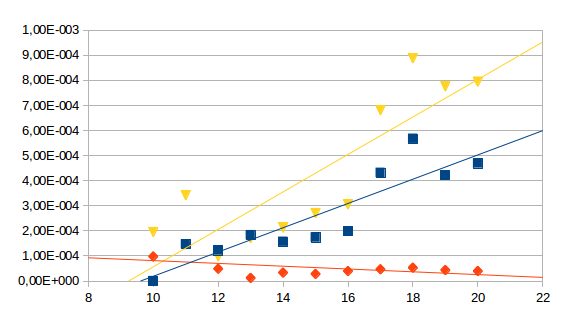
\includegraphics[width=0.8\textwidth]{freq1_ins}
  \caption{Tiempo inserci\'on para secuencia 1}
  \label{fig:f1}
\end{figure}

\begin{figure}[bp!]
  \centering
    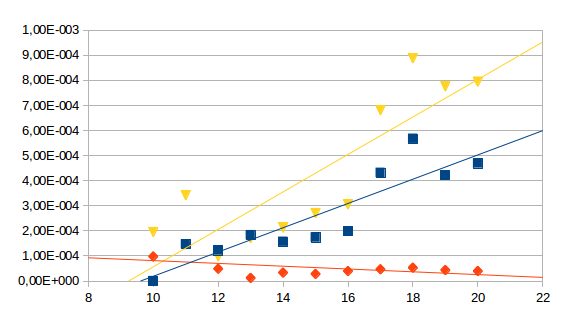
\includegraphics[width=0.8\textwidth]{freq1_busq}
  \caption{Tiempo b\'usqueda para secuencia 1}
  \label{fig:f2}
\end{figure}

\begin{figure}[bp!]
  \centering
    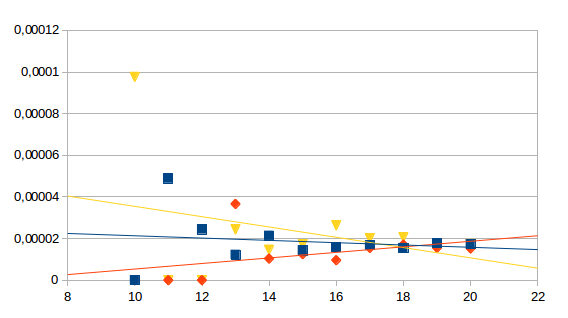
\includegraphics[width=0.8\textwidth]{freq215_ins}
  \caption{Tiempo inserci\'on para secuencia 2 y $a=1.5$}
  \label{fig:f3}
\end{figure}

\begin{figure}[bp!]
  \centering
    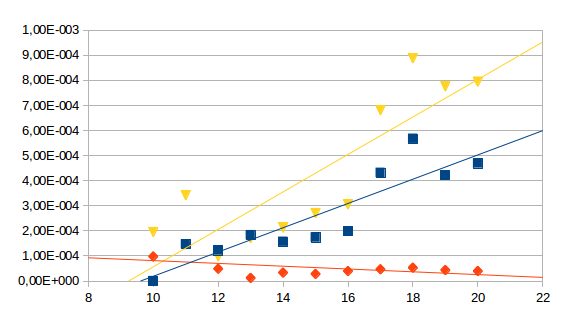
\includegraphics[width=0.8\textwidth]{freq215_busq}
  \caption{Tiempo b\'usqueda para secuencia 2 y$a=1.5$}
  \label{fig:f4}
\end{figure}

\begin{figure}[bp!]
  \centering
    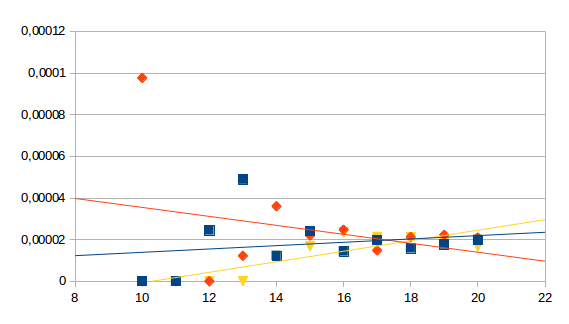
\includegraphics[width=0.8\textwidth]{freq320_ins}
  \caption{Tiempo inserci\'on para secuencia 2 y$a=2.0$}
  \label{fig:f5}
\end{figure}

\begin{figure}[bp!]
  \centering
    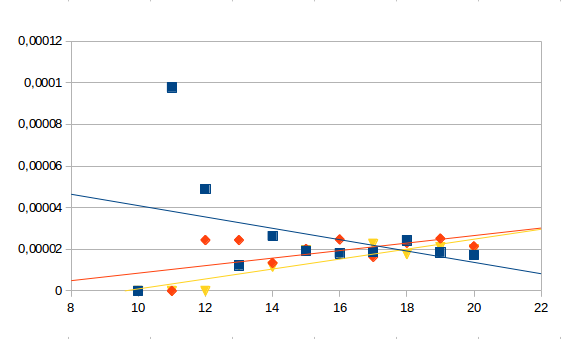
\includegraphics[width=0.8\textwidth]{freq320_busq}
  \caption{Tiempo b\'usqueda para secuencia 3 y$a=2.0$}
  \label{fig:f6}
\end{figure}
\fi
\newpage
\section{An\'alisis e Interpretaci\'on de Datos}
 \subsection{Inserciones}
 
Podemos ver que para el caso de datos generados la cantidad de I/O's y el tiempo a medida que crece $n$, es lineal para ambos casos de inserción(\textit{LinearSplit} y \textit{QuadraticSplit}). Sin embargo, podemos notar que para el caso de \textit{LinearSplit} este toma casi la mitdad del tiempo que \textit{QuadraticSplit}. Ademas \textit{LinearSplit} hace ligeramente menos I/O's que \textit{QuadraticSplit}.

Por otro lado, en el caso en que los rectángulos son generados a partir de datos reales. Vemos que nuevamente el tiempo de inserción para el método \textit{LinearSplit} toma bastante menos tiempo que textit{QuadraticSplit}. Sin embargo, en la cantidad de I/O's ambos algoritmos se comportan relativamente similar.

Dado la naturaleza de ambos algoritmos de inserción es fácil ver que para el caso de \textit{LinearSplit} este iba a lograr menores tiempos de inserción en comparación a \textit{QuadraticSplit}. Esto se debe a que la naturaleza de su algoritmo hace generar arboles mas irregulares. Es decir, genera arboles menos balanceados que \textit{QuadraticSplit}. Esto se debe a que las estrategias de \textit{LinearSplit} son mas laxas. Sin embargo, esto puede producir que al momento de realizar operaciones sobre un árbol generado por \textit{LinearSplit} esta tome mas tiempo que en \textit{QuadraticSplit}.

 
\subsection{Búsqueda}
Lamentablemente después de analizar ambos casos, Datos reales y generados. Se puede concluir que el método de búsqueda posee algún error. Se cree que este no estaba cargando los datos de disco por lo tanto al leerlos de memoria primaria arroja los datos adjuntos. Que son de costo prácticamente cero para ambos casos, que es de esperarse si los datos son leídos de memoria primaria.  

Por otro lado se esperaba que \textit{QuadraticSplit} tuviese mejores tiempos y menores I/O's que \textit{LinearSplit}.
 
\end{document}
